\subsection{Simplified and original Ikeda method}
\label{se:si_ikeda_model}
Since the agreement between the SI-method and the reference model test result was not very good a second study was conducted to see if the original Ikeda method would give better results. In the Ikeda method more detailed information about the ship hull geometry is needed so that $B_W$ can be calculated with a strip method and $B_E$ can be calculated using sectional lewis coefficients. It was possible to collect the required hull inputs for 14 ships in the database. Scale models of these ships were used in 46 of the reference roll decay tests.

\begin{figure}[H]
    \centering
    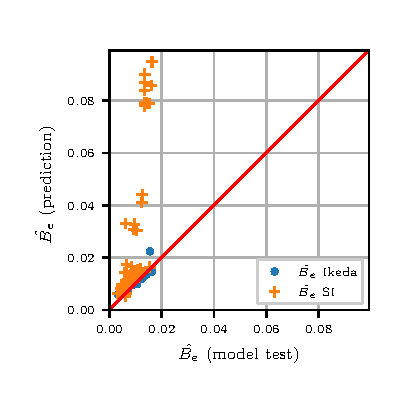
\includegraphics[]{figures/si_ikeda_model.eps}
        \vspace{-0.5cm}
    \caption{Comparison SI, Ikeda and model tests}
    \label{fig:si_ikeda_model}
\end{figure}
